\section{Workflow Overview} % (fold)
\label{sec:workflow_overview}

This section provides a brief overview of how MiCS works. Figure \ref{fig:mics_internal_workflow} shows the stages that MiCS goes through when converting C\# to JavaScript.

\begin{figure}[H]
	\begin{center}
		\centerline{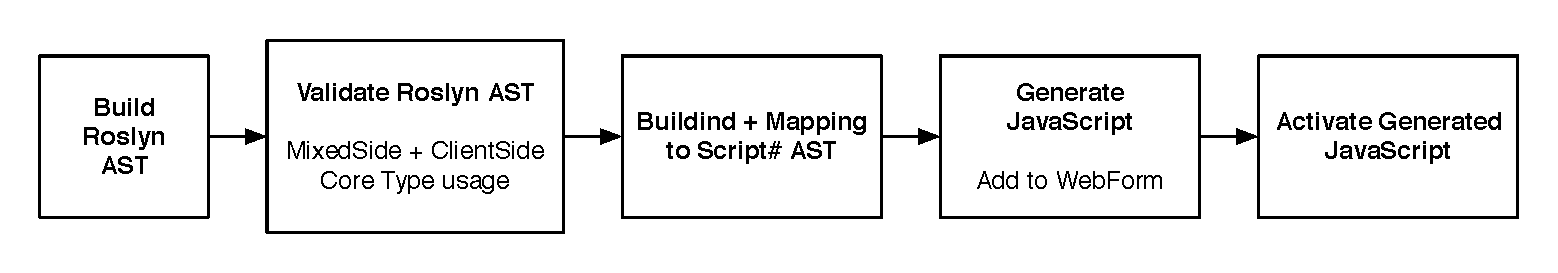
\includegraphics[width=18cm]{resources/images/internalworkflow.eps}}
	\end{center}
	\caption{MiCS generate an AST representing the user's C\# code. This AST is validated and mapped to a Script\# AST, that represents JavaScript. From the Script\# AST, JavaScript is generated and finally added to the user's web page.}
	\label{fig:mics_internal_workflow}
\end{figure}

MiCS uses Roslyn to generate a C\# AST representing user's  C\# code. Apart from the C\# AST, a Roslyn Semantic Model is also generated to obtain type information on AST nodes. The Semantic Model includes information on user types and referenced types.

When the Roslyn AST has been obtained it needs to be validated to ensure that the written code complies with the Mixed Side Principle and that core types are only used in a supported manner. Without validation, it would be possible for the user to generate incorrect JavaScript.

Once the syntax tree has been validated, it is ready to be mapped to the Script\# AST. This is the core functionality of MiCS - transforming a Roslyn AST to a Script\# AST. During the mapping process it is checked that the user does not utilize any C\# constructs that is not support by MiCS. 

When the Roslyn AST has successfully been mapped to a Script\# AST, MiCS utilizes Script\#’s built-in ScriptGenerator to generate the JavaScript corresponding to the user’s original C\# code. 

When JavaScript has been generated, it needs to be embedded into the user’s web page. Client side event handlers needs to be registered so that the generated JavaScript will be executed.


% section workflow_overview (end)